\documentclass[5pt,a4paper]{article}
\usepackage[utf8]{inputenc}
\usepackage{amsmath}
\usepackage{amsfonts}
\usepackage{amssymb}
\usepackage{graphicx}


\begin{document}


\begin{titlepage}
    \begin{center}
        \vspace*{1cm}
        
        \Huge
        \textbf{Planning Summary}
        
        
        \vspace{1.5cm}
        
        Author:
        \textbf{Nicolò Brandizzi}\\
        \vspace{0.5cm}
        \Large
        Contributors:
        \textbf{}%add contributors here
        
        \vfill
        
        
\includegraphics[width=0.4\textwidth]{images/sapienza_logo.jpg}


        
        \vfill
        
  

        \vspace{0.8cm}
        
        
        \Large
        DIAG\\
        Sapienza\\
        October 2018

    \end{center}
\end{titlepage}


\tableofcontents
\newpage
\begin{abstract}
This is \textbf{free} material! You should not spend money on it.\\
Find the complete material on GitHub \url{https://github.com/nicofirst1/AI_notes}.

This notes are about the \textit{Planning} part taught by professor Daniele Nardi in the Artificial Intelligence class. Everyone is welcome to contribute to this notes in any relevant form, just ask for a pull request and be patient.\\ Remember to add your name under the contributors list in the title page when submitting some changes (if you feel like it).
\end{abstract}
\newpage

\section{Classical Planning}
A plan is a sequence of actions that allows us to reach a state where the goal condition holds, starting from the initial state.\\
For a classical planning problem we need to define 3 things:
\begin{itemize}
\item States, which are represented by \textit{sets of instantiated literals} with a boolean value
\begin{itemize}
\item Initial State
\item Goal State
\end{itemize}

\item Actions or \textbf{action schema} composed of:
\begin{itemize}
\item Action name
\item List of variables used in the schema
\item A precondition : define the state in which the action can be executed
\item An effect : result of an action
\end{itemize}
\item An Environment:
\begin{itemize}

\item Fully observable
\item Deterministic
\item Static
\item Discrete and Finite
\end{itemize}
\end{itemize}


Obviously an action can be executed in a state if the state \textit{entails} the preconditions, i.e. the action is \textbf{applicable} in the state.\\

Lets consider the following example:

\begin{itemize}
\item Initial state: \textit{Plane 1 in A}
\item Goal state: \textit{Plane 1 in B}

\item Action: \textit{Fly(Plane,From, To)}
\begin{itemize}
\item Precondition : \textit{Plane in From}
\item Effect: \textit{Plane at To}
\end{itemize}
\end{itemize}

If we use the action \textit{Fly(1,A,B)} the following thing happen:

\begin{itemize}
\item The plane is not in A anymore, so \textit{At(1,A)} is deleted and added to the \textbf{delete list} [DEL(a)]
\item The plane is in B, so now \textit{At(1,B)} is true and is added to the \textbf{add list} [ADD(a)]
\end{itemize}

Intuitively we have that the precondition always refer to the time \textit{t} while the effect refers to the time \textit{t+1}.

\paragraph{Complexity of classical Planning}

We refer to:
\begin{itemize}
\item \textbf{PlanSAT} as the question to whenever it exist any plan that solves a planning problem, which is decidable for finite states, but becomes semi-decidable if we add function symbols to the language\footnote{The consequence is an infinite space}.
\item \textbf{Bounded PlanSAT} as whenever there is a solution of length $k$,which remains decidable even with infinite states.

\paragraph{Forward state-space search}
Apply actions whose preconditions are satisfied unitl goal state is found or all states have been explored \footnote{Mapping planning into a search problem}, with the following consequences:
\begin{itemize}
\item $Results(s,a)=(s-DEL(a))\cup ADD(a)$
\item The exploring of irrelevant actions
\item The issue for the large space this kind of problems have.
\item Strong domain-independent heuristics can be derived automatically.
\end{itemize}

\paragraph{Backward relevant-state search}
If a domain can be expressed in PDDL then we can do regression on it \footnote{This is because we keep in memory both the DEL(a) and the ADD(a) lists}. If we want to go from the goal $g$ with an action $a$ to the state $g'$ we have:
\[g'=(g-ADD(a)) \cup Precond(a)\]
We can do this as long as an action $a$ is \textbf{relevant} to the state $g$. Regression keeps the branching factor low, but it makes harder to come up with good heuristic, thus forward is preferred.


\paragraph{Heuristic for Planning}
Remember that an admissible heuristic can be derived from the \textbf{relaxed problem} which is easier to solve.\\
Search problems can be seen as a graph where nodes are stated and edges are actions. There are three ways you can relax a problem with graph:
\begin{itemize}
\item \textbf{Ignoring preconditions}: drop all precondition of an action. Usually this means that the number of actions to solve the problem is the same as the number of unsolved goal. On the other hand if we may have actions which achieve multiple goals or actions which  can undo other actions \footnote{Can be ignored to relax the problem}. .

\item \textbf{Ignore delete list}: remove all negative literals from effects \footnote{No action can undo the progress made by another action.}, monotonic progression towards the goal.

\item \textbf{State abstraction}: many-to-one mapping where we decrease the number of states by ignoring some fluent.

\item \textbf{Decomposition}: dividing the problems into parts and solving them independently \footnote{Assume sub-goal independence}, but it is a pessimistic approach \footnote{Not admissible} when sub-plans contains redundant actions.

\end{itemize}

\paragraph{Lemma}
If the effect of $P_i$ leaves all the preconditions of $P_j$ unchanged, then the estimated cost $Cost(P_i)+Cost(P_j)$ is admissible and more accurate of the maximum.





\newpage

\section{Partial Order Planning [POP]}

Many sub-problems are independent so we can work on several sub-goals independently, solve them and then combine them to achieve a solution to the original plan.\\
A Partial Order Planner is a planning algorithm which can place two action into a plan without specifying which comes first, so that the solution is in the form of a \textit{graph} rather than a sequence.
POPs are created by a search in the \textit{space of plans} rather than through the state space, where an action is actually a plan \footnote{The difference is subtle. An action may be \textit{Move(what,where)} where a plan is \textit{Move(ObjA,Pos1}).}. They work by  \textbf{fixing flaws}\footnote{A flaw is anything that keeps the partial plan from being a solution} in the plan with the principle of \textbf{least commitment} \footnote{Delaying a choice during the search until it is strictly necessary.}. \\

Each plan has four components:

\begin{itemize}
\item A  \textbf{set of actions} that makes up the steps for the plan. An empty plan has only the \textit{Start} and \textit{Finish}  actions.
\item A set of \textbf{ordering constraints} between pairs of actions in the form $A\prec B$ (A happens some time before B).
\item \textbf{Causal links} $A \xrightarrow{\text{p}} B$ (A achieve $p$ for B) \footnote{For example when putting on shoes we may have $RightSock  \xrightarrow{RightSockOn} RightShoe$, meaning that putting the right sock on achieves the condition necessary for putting the right shoe on.}. The presence of causal links lead to \textit{early pruning} of portions of state space that, because of not resolvable conflicts, contain no solutions.

\item \textbf{Open preconditions}  for an action not yet causally linked, i.e. a precondition that is not achieved by any action yet. 
\end{itemize}

If a plan has the following proprieties than it is defined as \textbf{consistent}:
\begin{itemize}
\item All the open preconditions are achieved \footnote{A precondition is \textit{achieved} if no action can undo it's effects.}
\item There are no \textbf{cycles}, i.e. $A\prec B$ and $B \prec A$ which is also a contradiction.
\item There are no \textbf{conflicts}, that is when $A \xrightarrow{\text{p}} B$ and an effect of another action $C$ is $\neg p$ where  $A \prec C$ and  $C \prec B$. Note that a conflict can be solved by applying:
\begin{itemize}
\item A \textbf{Demotion} $C \prec A$
\item A \textbf{Promotion} $B \prec C$
\end{itemize}

\end{itemize}
A consistent plan with no open preconditions is a \textbf{solution}.\\

The algorithm works in the following way:
\begin{enumerate}
\item The plan only contains $Start$ and $Finish$ with $Start \prec Finish$
\item The successor function: 

\begin{enumerate}
\item pick an open condition $p$ of an action $B$
\item pick an action $A$ that achieves $p$
\item add the causal link $A\xrightarrow{\text{p}} B$ and $A \prec B$
\item resolves conflicts if possible, otherwise backtrack
\end{enumerate}
\item The goal test succeeds when there are no more open preconditions

\end{enumerate}


\newpage

\section{Non-Deterministic domains}

\subsection{Searching with Non-deterministic actions}
When the future percepts cannot be determined in advance \footnote{The state is only partially observable.} the solution to a problem is a \textbf{contingency plan}. In this case the \textit{result} of a problem is a function that return a \textbf{set} of possible outcomes states \footnote{Rather than a specific one.}. That is why the solution of a non-deterministic problem can contain nested \textbf{if-then-else} statements so that the form is \textit{tree-like} rather than a sequence.

\paragraph{And-or trees}
The branching of a tree can depend on:
\begin{itemize}
\item The \textbf{agent's choices}, which will generate OR nodes
\item The \textbf{environment's choice}, which will generate an AND node.
\end{itemize}

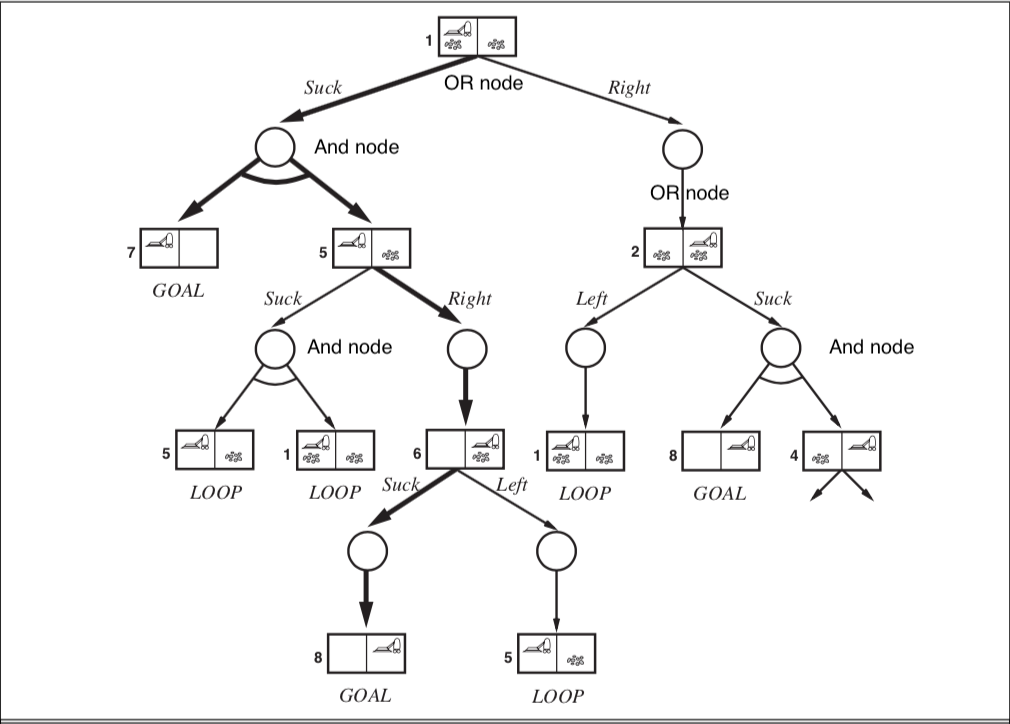
\includegraphics[scale=0.5]{images/And-or-tree.png} 

\paragraph{Non-cyclic Solutions} The issue is that cycles often arise in this kind of problem.We can consider a solution in which: if the current state is identical to a state on the path from the root, than return false. This method guarantee to terminate in every finite space and return a solution which is \textbf{non-cyclic}.

\paragraph{Cyclic Solutions}
When we deal with non-deterministic actions we can get to the point where an action must be repeated some times to make it work \footnote{Slippery floor for robot movement}. So we want to keep doing an action until some state is reached \footnote{Using \textit{while} conditions}. This leads to \textbf{cyclic solution} which will eventually reach the goal provided that each outcome of a non-deterministic action eventually occurs.




\subsection{Searching with partial observation}
For this kind of searching we need to introduce the concept of \textbf{belief state}, representing the agent's current belief about the possible physical states it might be in.

\paragraph{Sensor less belief} With a specific sequence of action an agent can \textbf{coerce} the world into a state $X$ \footnote{That is the agent is sure to be in $X$ after execution a sequence of actions}. Since the agent always know its own belief state we can derive that the latter is \textit{fully observable}, furthermore the solution (if any) is always a sequence of actions.\\
A sensor-less problem [P] has the following elements:
\begin{itemize}
\item \textbf{Belief states}: contains every possible set of physical states
\item \textbf{Initial state}: the set of all states in P
\item \textbf{Actions}: there are two cases which depends on their effect on the environment 
\begin{itemize}
\item \textit{Illegal action have no effect on the environment}: then we can take the \textbf{union} of all the actions in the current belief state
\item \textit{Illegal action have effect on the environment}: then we take the \textbf{intersection}
\end{itemize}


\item \textbf{Transition model}: The model which generate a new belief state $b'$ \footnote{Also called the \textit{prediction} step.}  from a belief $b$ troughs an action $a$, it depends on the type of action:

\begin{itemize}
\item \textit{Deterministic} action: $b'=Result(b,a)=\{s':s'=Result_P(s,a), s \in b\}$
\item \textit{Non-Deterministic} action: $b'=Result(b,a)=\{s':s'=Results_P(s,a), s \in b\}=\cup_{s\in b}Reulsts_P(s,a)$
\end{itemize}

\item \textbf{Goal test}: the belief state satisfies the goal only if all the physical states in it satisfy the $GoalTest_P$
\item \textbf{Path cost}: assumed same for every action
\end{itemize}

Since The size of each belief state is exponential we can use the \textbf{incremental belief-state search} in which we first find a solution that works for state 1; then check if it works for state 2; if not, go back and find a different solution for 1, and so on.

\paragraph{Searching with observations}
In this case we have the \textit{Percept(s)} function which returns the percept in a given state. When an observation is \textit{partial} then we could have it generated by several states.  In this case the difference with the sensor-less problem mentioned above are the following:
\begin{itemize}
\item There is a \textbf{prediction} stage.
\item There is a \textbf{observation prediction} stage in which we determine the set of percepts that could be obtained in the predicted belief state
\item The \textbf{update} stage, for each possible percepts we get the belief state that would result from it \footnote{Reduces uncertainty.}.
\end{itemize}


\subsection{Planning in Non-Deterministic domains}


For planning we augment the PDDL with a \textbf{precept schema}.\\
\textbf{Online planning} can generate a contingent plan with fewer branches at first, and deals with problems as they arise. While \textbf{re-planninig} agents would check the result and replan in case of unexpected failure.



\paragraph{Sensorless planning}
We can convert a sensorless problem to a belief-state planning problem where the transition model is represented by a set of action schemas and the belief model is represented by a logical formula \footnote{Instead of being all the possible enumeration of the states.}.\\
If an effect depend on the state then we have a \textbf{conditional effect} which is denoted like this:
\[\textbf{when}\quad condition: effect\]
This kind of effect brings the belief state to have an exponential size in the worst case.

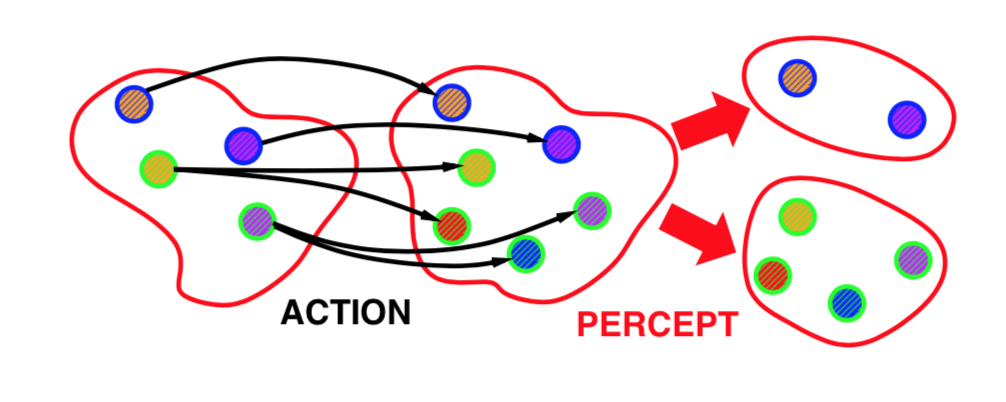
\includegraphics[scale=0.70]{images/belief_state.png}
The different between unsatisfied conditional effect and unsatisfied precondition is that the latter do not permit the action to occur, thus the resulting state is \textbf{undefined},while an unsatisfied conditional effect \textbf{does not change the state}.\\
Other kind of solutions can be:
\begin{itemize}
\item Perform some actions which keeps the belief state as simple as possible \footnote{Like when we check the time every once in a while to lower our uncertainty of the current time.} and lower uncertainty.
\item Not compute the belief state after some actions, but rather represent it as being followed by those action without computing it.
\end{itemize}
The final piece is to implement a good heuristic function to guide the search. Since any subset of the original belief is easier to solve we have that any heuristic which is admissible for a subset of the original belief state is also admissible for the entire belief state with the maximum function:
\[H(b)=max(h_1(b),...,h_n(b))\]



\subsection{Online replanning}

\paragraph{Execution monitoring}

Determine the need for a new plan. Some branches of a partially constructed contingent plan can simply say Replan; if such a branch is reached during execution, the agent reverts to planning mode. Replanning may occurs in the following situations:

\begin{itemize}
\item \textbf{Missing precondition}
\item \textbf{Missing effect}
\item \textbf{Missing state variable}
\item \textbf{Exogenous events}: changes in the goal
\end{itemize}

\paragraph{Action Monitoring}
Before executing an action, the agent checks if all the preconditions still hold.
\paragraph{Plan Monitoring}
Before executing an action, the agent verifies that the remaining problem will still succeed. It can detect failure by checking the preconditions for success of the entire remaining plan. It cut off the execution of a dead plan as soon as possible and it also allows \textbf{serendipity} \footnote{Accidental success.}. 
\paragraph{Goal Monitoring}
Before executing an action, the agent checks if there is a better set of goals it could try to achieve.

\end{itemize}



\newpage



\newpage

\section{High-level actions}

We introduce the concept of \textbf{high-level action} [HLA] which is part of the \textbf{hierarchical task networks} [HTN] which assumes the full \textit{observability}, \textit{determinism} and \textit{availability} of a set of actions called \textbf{primitive actions}.\\
A \textbf{refinement} is a sequence of actions which describes \footnote{Or decomposes.} an HLA. If a refinement contains only primitive actions then it is called \textbf{implementation}.\\ A high-level plan achieves the goal from a given states if at least one of its implementations achieves the goal from that state.\\A set of possible implementations in HTN planning is not the same as a set of possible outcomes in non-deterministic planning.

\subsection{Searching for primitive solutions}
It always start with a top level action called \textbf{Act}, then, for each primitive action $a_i$, we provide a refinement of Act with steps $[a_i,Act]$. The algorithm then becomes one that repeatedly chooses an HLA in the current plan and replace it with one of its refinements until the goal is achieved. This is computationally expensive, given:
\begin{itemize}
\item $d$ primitive actions
\item $b$ allowable actions at each state
\item $k$ actions 
\item $r$ possible refinements
\end{itemize}


The possible decomposition trees are:
\[r^{\frac{d-1}{k-1}}\]
Which, by taking small $r$ and large $k$ \footnote{Small number of refinements each yielding a large number of actions.} , results in huge savings.\\
Some algorithms may even save successful plans in memory to later build newer plans on top of the older ones, leading to a more competent planner over time \footnote{The problem lays in generalizing the methods that are constructed.}.

\subsection{Searching for abstract solutions}
If we write precondition-effect description for an HLA we can check whenever an HLA achieve goal without decomposing it with the refinements. So an HLP must have at least one implementation that achieves the goal to be considered doable, this is called the \textbf{downward refinement property}.\\
The problem lays in the description of the effect of an action which can be implemented in many different ways. A solution might be to include only the positive effects that are achieved for \textit{every} implementation of the HLA and the negative effects of \textit{any} implementation.\\
We introduce the notion of \textbf{reachable set} for an HLA $h$ \footnote{Written Reach(s,h)} in a state $s$, the set of states reachable by any implementation of HLA. We can now say that a sequence of HLAs achieves the goal if its reachable set intersect the set of goal states.

\paragraph{Angelic semantics} 
Given a \textit{fluent} \footnote{A state varaible}, a primitive action can add, delete or leave unchanged a fluent. The HLA under angelic semantics can control the fluent's value depending on which implementation is chosen.\\
For example to HLA \textit{Go(home,work)} with two possible refinements:
\begin{itemize}
\item Drive(home,work)
\item Call(taxi),Taxi(home,work)
\end{itemize}
can have as requirement for the $Taxi$ action to have $Cash$. Under angelic semantics the agent can choose to delete $Cash$.\\
This results in the derivable descriptions of HLAs from their refinements.\\
The angelic approach can be extended to find the least-cost solution by introducing the most efficient way to get to a state.

\paragraph{Descriptions}
There are two kind of descriptions which are kind of a upper/lower bound for the reachable set:
\begin{itemize}
\item \textbf{Optimistic}: may overstate the reachable set of an HLA 
\item \textbf{Pessimistic} : may understate the reachable set.
\end{itemize}
We can derive that if an optimistic reachable set does not intersect the goal then the plan does not work, on the other hand if a pessimistic description set intersect the goal then the plan works for sure. Additional refinement is needed when the optimistic intersects but the pessimistic doesn't.











\end{document}
